

\documentclass[12pt, titlepage]{article}

%% preamble: Keep it clean; only include those you need
\usepackage{amsmath}
\usepackage[margin = 1in]{geometry}
\usepackage{graphicx}
\usepackage{booktabs}
\usepackage{natbib}
\usepackage[table]{xcolor}
\usepackage{booktabs}

% for space filling
% highlighting hyper links
\usepackage[colorlinks=true, citecolor=blue]{hyperref}


%% meta data
\setlength\parindent{24pt}
\linespread{2}
\title{WNBA vs NBA Earnings In Comparable Players}
\author{Colin Sullivan\\
  Department of Statistics\\
  University of Connecticut
}

\begin{document}
\maketitle

%   \begin{center}
%       \vspace*{1cm}
%       \Huge
%       \textbf{How to Earn a Salary}
%
%       \Large
%       \vspace{0.5cm}
%        A Closer Look at WNBA and NBA Player Salaries, the Discrepancies, and What Statistics Might Influence Them
%            
%       \vspace{1.5cm}
%
%       \textbf{Colin Sullivan}
%       
%       \vfill
%
%
%       \vfill
%            
%            
%       \vspace{0.8cm}
%     
%         
%        \Large    
%       Department of Statistics\\
%       University of Connecticut\\
%       Storrs, CT\\
%            
%   \end{center}
\newpage

\begin{abstract}
In a world where gender pay gaps have been highlighted in nearly every industry, professional sports are no exception. The Women’s National Basketball 
Association is widely known and accepted to pay very significantly less annually to its players than the male league counterpart, the National Basketball 
Association. There has been a lot of research into this pay gap, and this paper will look to add to the conversation by examining the structure of 
contracts in relation to performance. This will be done using statistics from the 2018 seasons of each respective league, using datasets cleaned up and 
analyzed with various Python scripts to eventually draw conclusions on the relation between performance and pay for male and female athletes.	
\end{abstract}

\section{Introduction}
\hspace*{10mm}
Since the formulation of the Women’s National Basketball Association (WNBA) in 1996, there have been never-ending debates among fans comparing the female 
league to the much older, more popular National Basketball Association (NBA). Women’s basketball has a rich history marred by frequent sexism, fewer 
opportunities, and significantly less financial support.
\par
Women’s basketball began being played in 1892 at Smith College, just one year after men’s basketball was invented \citep{Shattering_The_Glass}. Due to the 
gender roles and cultural norms of the time, however, women were believed to be very fragile and unable to play physical sports like 
basketball at anywhere near the same level as men. As such, women played under modified rules specially created for them \citep{WNBA_Hist}. Those familiar 
with basketball will know that it is usually played competitively with 5 players on each team, and each player runs the full court to play offense on one 
end and defend the other team on the other. In 1892, however, women initially played “9 on 9”, with the court divided into three areas: offense, 
defense, and mid-court. Each player was assigned to play within one of these cours, such that 3 women on each team were in each section. The 
players could not leave their section of the court to go into the other, essentially creating three separate “3 on 3” games. The other major rule change 
from Naismith's game was that women could only dribble the ball a limited number of times and could not hold it for more than three seconds, a rule 
attributed to the fear that the players might suffer “nervous fatigue” if the game were too strenuous \citep{WNBA_Hist}.
\par
The gradual changing of perspectives on women’s athletics is seen in the evolution of women’s basketball; while the game of men’s basketball has largely 
stayed the same over the course of its almost 130 year history (key changes including the legalization of the slam dunk and the implementation of the 
three point line), women’s basketball has shifted slowly to eventually become almost identical. The sport was played inter-collegiately for decades 
beginning in the late 19th century, but did not enter the professional realm until the 1970s. Women's basketball became officially recognized at the collegiate 
level by the NCAA in 1982 (a shockingly late introduction), and the Women’s Basketball League (WBL), founded in 1978 and only lasting three seasons, was 
the first of several failed women’s professional leagues in the late 20th century. Meanwhile, the NBA experienced a huge boom in popularity largely due to 
the emergence of superstars Larry Bird, Magic Johnson, and Michael Jordan. The massive increase in NBA reach and revenue directly led to the league 
creating, funding, and supporting the WNBA in 1996.
\par
There are minimal differences between today's women’s basketball and the basketball that men have been playing since inception. The WNBA and women's 
collegiate ball is slightly smaller than that used by male players, the three point line is a foot to two feet shorter, and the game clock features 
four 10 minute quarters as opposed to the NBA’s 12 minute quarters. Nevertheless, for all intents and purposes the games are the same. The rules are otherwise 
identical, the athletes are similarly talented, the level of play is incredibly high, and the games are very enjoyable to watch. There remains only one 
massive difference between the two leagues: player salaries.
\par
The difference in player salaries is a huge point of contention in women’s basketball discourse and is often the subject of intense ridicule, and it is 
easy to see why: top NBA players make upwards of 40 million USD per season, not including endorsement deals and other income, while the WNBA most valuable 
player makes less than the average office worker in New York (an exaggeration, maybe, but Elena Delle Donne made around 120 thousand USD in her MVP year 
with little extra endorsement money or exposure). An NBA rookie signs one contract and has enough wealth to live comfortably off for the rest of his life, 
often for generations; a WNBA prospect is encouraged to continue her academic studies to ensure that she is able to get a well-paying job after her career 
is over. Now, granted, the league revenue is much much less than that of the NBA, but many questions still remain that this paper hopes to address: Are 
the players paid fairly compared to league revenue? Are they compensated equally based on basketball production? How can this change?
\par
There have been numerous studies surrounding that of the NBA and the WNBA and the differences in salaries.
For example, one such paper authored by Elle Baker discusses the intra-league salary distribution and
how WNBA players, despite getting paid far less, have much less "salary inequality"
\citep{baker2020comparison}. Another argues for an increase in salaries in the WNBA (a cause everyone
should be able to get behind) by citing the league's growth in fans and revenues \citep{ettienne2019s}. A third paper, by Ball State statistics student 
Alyssa Bridge took a close look at media tie ins to the WNBA and found that, among other inequalities, only 2\% of ESPN’s SportsCenter airtime is devoted 
to discussing it. \citep{Bridge}
This paper hopes to build off some of the research done by Hailey DiCicco in "Hoop Dreams: An Empirical Analysis of the Gender Wage Gap in Professional 
Basketball". DiCicio performed regression analysis on the correlation between win percentage and team performance in basic statistics (rebounds or steals, 
for example). She was, however, unable to come to any significant conclusions beyond that of basic comparisons of salaries \citep{Hoop_Dreams}.
\par
This paper will not compare just salaries of WNBA vs NBA players, which is something that has been done numerous times, but will go further in depth and 
examine the correlation between individual player pay and performance in numerous advanced statistics. The goal is to draw conclusions on if there 
are certain statistics in the NBA that result in higher adjusted salaries than the WNBA and vice versa, what the correlation is between them, and 
determine "superstar" salary factors.
\par
Immediately following this section, this paper will discuss the datasets being analyzed and how they were cleaned and prepped for analysis using Python 
scripts. In the next section, statistical analysis will be performed to try and answer some of the questions posed in this introduction. Following that 
will be a discussion on the results and hypotheses for best paths forward. Finally, there will be a conclusions section to wrap up the paper and review 
the results.


\section{Data}
\hspace*{10mm}
There are two primary data sets that I will be using to conduct the analysis in this paper. The first of these is a database of historical WNBA data 
dating from 2001-2020, collected by Neil Payne, sports editor at 538, and displayed on his GitHub account \citep{first}. Unlike most data sets, this one 
contains a multitude of advanced statistics for each player.

\par
Using another data set from Paine’s Github, a Python script called WNBA\_Cleanup.py was written and used to combine salary data from the two sources and 
filter out the desired candidate players from the data set. This paper will focus on comparing players from the 2018 NBA and WNBA seasons, so that filter 
was applied. The script also filtered out players who played less than 5 games and those that did not have salary data, so as to make the set as 
standardized as possible and remove outliers. The final data set after filtration and combination was called WNBA\_Combined.csv and has data (the 
aforementioned statistical categories) for 166 WNBA players from the 2018 season.
\par
A corresponding NBA dataset was found, this time belonging to Mustafa Baris Camli on the data-sharing site Kaggle \citep{nba}. This data set contains a 
list of all players from the NBA in the 2017-18 season, with similar advanced statistics to the WNBA dataset. The statistics found in the datasets can be 
seen in \ref{tab:stats}.

\begin{table}[tbp]
    \caption{Statistics From the Datasets}
    \label{tab:stats}
\centering
\begin{tabular}{crr}
\toprule

Common Statistics & WNBA Exclusive & NBA Exclusive\\ 
\midrule
 Player Name  &  Team Net Rating & 3 Point Attempt Rate  \\
 Age &  Composite Rating & Offensive Box +/-      \\ 
 Position &  Wins Generated & Defensive Box +/-\\
 Team &  & Box +/-     \\         
 Minutes Played &  & VORP       \\
 Player Efficiency Rating & &      \\
 True Shooting \% & & \\
 Free Throw Rate & &\\
 Offensive Rebounding \% & & \\
 Total Rebounding \% & & \\
 Assist \% & & \\
 Steal \% & & \\
 Block \% & & \\
 Turnover \% & & \\
 Usage \% & & \\
 Offensive Win Shares & & \\
 Defensive Win Shares  & & \\
 Win Shares & & \\
 Win Shares per 40 games & & \\
 Salary & & \\
 
 \bottomrule
\end{tabular}
\end{table}

\par
The data set notably did not contain player salaries, so a second NBA data set was necessary. One was found on GitHub, created by Erik Gregory Webb, which 
contains the player salaries for every NBA player from 2000-2020 \citep{nba_salaries}. In a similar manner to the WNBA data, a Python script called 
NBA\_Cleanup.py was created to combine the data from the two datasets into one csv file. The data was then cleaned up by removing outliers (players 
playing under 5 games) and those that did not have salary data. The script was also used to combine data for players who played on multiple teams; the 
original data set would have players listed separately for each team they played on. The final data set after filtration and combination was called 
NBA\_Combined.csv and has data (the aforementioned statistical categories, plus player salaries) for 376 NBA players from the 2017-18 season.
\par
Finally, in order to compare the players accurately, the goal of checking their stats and salaries against league revenues must be achieved. As such, it 
was found that the NBA league revenue from 2018 was 8.01 billion USD \citep{NBA_Revenue} and the WNBA league revenue from the same year was 60 million USD 
\citep{WNBA_Revenue}.

\section{Research Design and Methods}
\hspace*{10mm}
Initially, we began by performing a paired sample t-test to confirm some expectations from the data. We do not need to perform a test to 
determine if NBA players are paid more than WNBA players, as that is commonly known and very obvious. As $\textit{Forbes}$ basketball author David Berri 
discovered, in general WNBA players are still paid significantly less than NBA players proportional to league revenue \citep{WNBA_Revenue}. In order to 
confirm that the data for the 2018 seasons fit with this mold, an initial t-test was performed:
$$H_0 = \mu_1 \leq \mu_0, H_a = \mu_1 > \mu_0$$
where $\mu_0$ represents the average WNBA salary proportional to league revenue and $\mu_a$ represents the same for the NBA. The test was done using a 
significance level of  5\%, or an alpha value of 0.05, and degrees of freedom $n_1 + n_2 - 2 = 516$. By the t-statistic chart, it must be checked if the 
found t-statistic is greater than 1.646. Using a Python script, Comp\_t\_tests.py, it was found that our t-statistic was 16.56. Since we want to convert 
this into a one tailed test, we halve the t-statistic to get 8.28, which is far greater than 1.646, so it can safely be said with 95\% confidence that our 
data follows the trend found in Berri's article.
\par
The primary focus of the analysis section was to analyze correlation using linear regression between advanced statistics and salary. This was done once 
again using python scripts: LR\_Test\_WNBA and LR\_Test\_NBA, for the WNBA and NBA, respectively, were used to read the data from the cleaned datasets and 
conduct simple linear regression analysis on all the advanced stats against player salaries. Then, using the scipy and matplotlib Python packages, each 
comparison was graphed with a line of best fit and a correlation coefficient ($R^2$) was found. This correlation coefficient tells us how strong the 
correlation effect is between the statistic and salary, which will help us draw significantly more accurate conclusions from the data then if simply the 
slope was examined. There were twelve overlapping statistics between the WNBA and NBA datasets, and the correlation coefficients for these statistics in 
both leagues are shown in \ref{tab:main_data}, with the standard error in parenthesis.


\begin{table}[tbp]
    \caption{WNBA vs NBA Correlation Coefficients For Selected Advanced Statistics}
    \label{tab:main_data}
\centering
\begin{tabular}{crr}
\toprule

Statistic &  CC: WNBA   & CC: NBA \\ 
\midrule
 PER  &  0.019458 (1.576)  & 0.25444 (0.014) \\
 FTr   &  0.001641 (0.036)  & 0.033096 (0.009)       \\ 
 ORB\%   &  0.019717 (0.929)  & 0.000274 (0.273)       \\   
 TRB\%   &  0.000017 (1.080)   & 0.007801 (0.337)       \\
 AST\%   &  0.041707 (1.936)  & 0.110984 (0.608)    \\
 STL\%  &  0.003666 (0.175)  & 0.006126 (0.045)       \\    
 BLK\%  & 0.000444 (0.337)   & 0.000141 (0.114)     \\
 TOV\%  & 0.010470 (1.432)  & 0.004207 (0.315)    \\
 USG\%   & 0.033326 (1.146)   & 0.202527 (0.350)       \\
 OWS   & 0.117693 (0.276)   & 0.337278 (0.121)        \\
 DWS  & 0.151183 (0.133)   & 0.234252 (0.068)         \\
 WS   &  0.153999 (0.365)  & 0.364165 (0.164)                 \\
 (WS/40)/(WS/48)   &  0.047009 (0.022)  & 0.151640 (0.004) \\
 \hline
 Sample Size & 142 & 376\\
 \bottomrule
\end{tabular}
\end{table}


\par
The graphs for the strongest correlation in both leagues (both the win shares statistic) are shown in figures \ref{fig:NBA_WS} and \ref{fig:WNBA_WS}.

\begin{figure}[tbp]
  \centering
  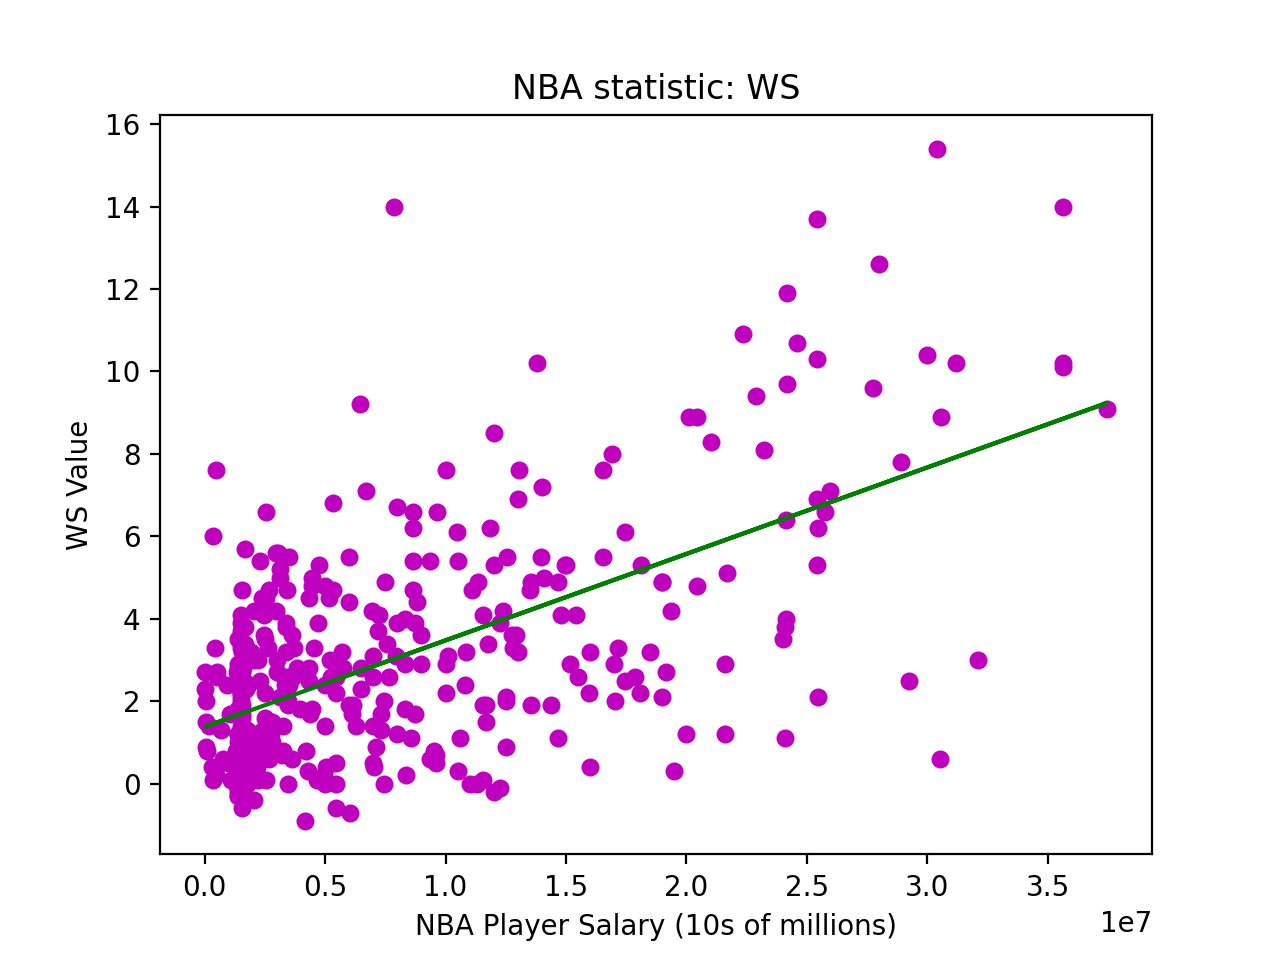
\includegraphics[width=.75\textwidth]{NBA_WS_Graph.png}
  \caption{NBA Player Salaries vs Win Share Performance.}
  \label{fig:NBA_WS}
\end{figure}
\begin{figure}[tbp]
  \centering
  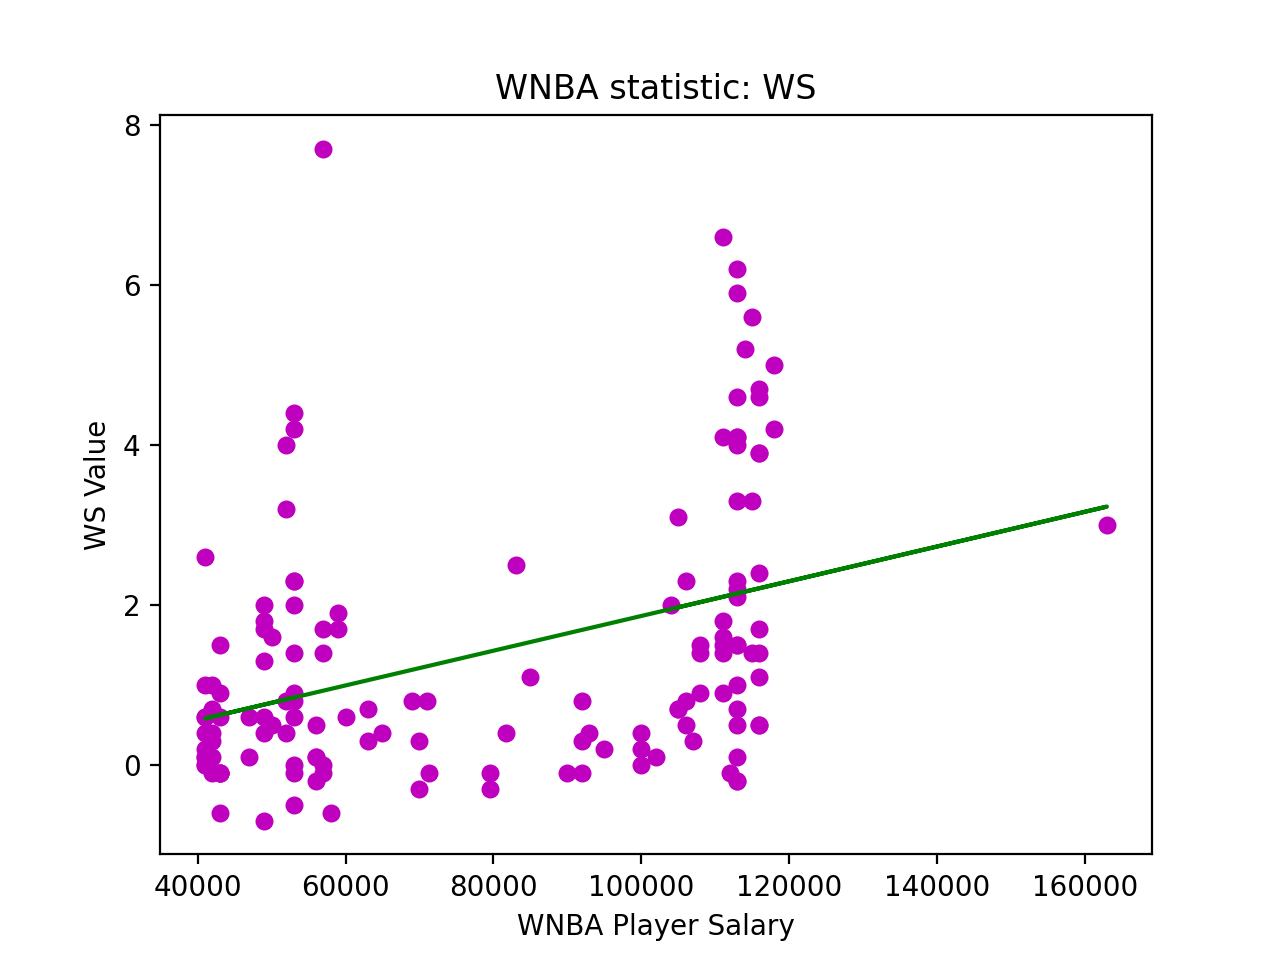
\includegraphics[width=.75\textwidth]{WNBA_WS_Graph.png}
  \caption{WNBA Player Salaries vs Win Share Performance.}
  \label{fig:WNBA_WS}
\end{figure}



\par
Finally, within the Comp\_t\_tests.py Python script, analysis was conducted on the salaries of the top players in each league. Instead of looking at 
simple statistics, work that has been done by DiCicio \citep{Hoop_Dreams}, this method used the advanced statistics from the data set. Six statistics were selected: Minutes 
Played (MP), Player Efficiency Rating (PER), Free Throw rate (FTr), Offensive Win Shares (OWS), Defensive Win Shares (DWS), and Win Shares (WS). The 
script was written to sort the datasets by these statistics, and the top 10 players in each league in these statistics were extracted. Then the salaries 
were compared to each respective league's median salary, and the average of these top 10 players relations to the average were compiled. The entries in 
the graph can be interpreted as follows: If the value is greater than 1, than the top 10 players in that statistic are paid the value as a factor above 
league average. If the value is less than 1, than the top 10 players in that statistic are paid the value as a factor below league average. The chart is 
shown in \ref{tab:top10}.

\begin{table}[tbp]
    \caption{How Much Compared to Avg the Top 10 Players Are Paid For Advanced Stats.}
    \label{tab:top10}
\centering
\begin{tabular}{crr}
\toprule
Statistic &  WNBA  & NBA \\ 
\midrule
 MP  &  1.445  & 5.353 \\
 PER   &  1.254   & 5.608        \\       
 FTr   &  1.087   & 2.053       \\         
 OWS   & 1.445    & 5.666        \\
 DWS  & 1.435    & 3.462       \\
 WS   &  1.530  & 5.446        \\
 \bottomrule
\end{tabular}
\end{table}




\section{Discussion}
\hspace*{10mm}
The data found from the initial t-test supported what had been found in the current literature. It was confirmed that in our 2018 data WNBA players are 
paid significantly less than NBA players, a known fact. It was also confirmed with a very high degree of certainty that WNBA players are paid less than 
NBA players proportional to league revenue (around 60 million for the WNBA, 8 billion for the NBA). This confirms the findings of David Berri \citep{WNBA_Revenue}, and was found 
to be particularly interesting while being generally intuitive based upon the narrative surrounding pay in women’s basketball.
\par
The main focus of the research was the regression analysis. Simple linear regression was used to create $R^2$ correlation coefficients for every advanced 
statistic in the WNBA and NBA datasets compared to player salaries. Since the base salary and proportional salary in the leagues are so different (as 
shown in the aforementioned t-tests), it seemed most appropriate to simply see which statistics correlated the strongest to salary increases. \ref{tab:main_data} 
shows the selection of correlation coefficients for the thirteen matching statistics between the two league data sets.
\par
Surprisingly, the correlation coefficients for almost every statistic was very low. For certain less consequential statistics (like Free Throw rate) this 
discovery was not shocking, but for more relatively important ones like Win Shares / Minutes it was interesting to see such low correlation between 
performance and pay. That being said, of the most important statistics - Player Efficiency Rating and Win Shares (including the Offensive and Defensive 
Win Shares sub statistics) - the NBA saw a significant increase in correlation coefficient, with all being above 0.23. The WNBA, on the flipside, did not 
see such an increase: Player Efficiency Rating had an extremely small coefficient, and while WS, OWS and DWS were all higher than other statistics, they 
still capped out at 0.15, lower than 6 of the NBA statistics coefficients. The graphs for the two highest correlations, Win Shares, are shown, and it can 
be visibly seen that higher performance in the NBA leads to higher pay more often than in the women’s counterpart league.
\par
The visual distribution of pay vs performance in figures \ref{fig:NBA_WS} and \ref{fig:WNBA_WS} is particularly interesting. While the correlation coefficient for both the WNBA and the NBA 
when compared to Win Shares is relatively high, the NBA graph looks much more traditionally distributed: Examining it finds the data generally following 
the trend line. The WNBA figure \ref{fig:WNBA_WS}, however, looks much less traditional. It forms a sort of "U" shape, where players are almost all clustered into two salary 
buckets which are distributed similarly over the y axis. While there are more "higher performing" players in the higher pay bucket, the distribution is 
nevertheless strange to see.
\par
Finally, some data manipulation was done to find a more simple statistic to try and determine how excellence in a statistic impacts pay. As \ref{tab:top10} shows, 
there is a much clearer trend in performing in the top 10 in a statistic and a pay increase. As the WNBA pay spread is much smaller than the NBA’s it is 
expected that there will be less of an increase. An encouraging sign is found in this table: finishing top 10 in every statistic (with the exception of 
Free Throw rate, the least consequential of the statistics) led to a significant pay increase in both leagues. The NBA consistently saw an increase of 
over 5 times league median salary, while the WNBA hovered around 1.5 times league median.
\par
None of the data found is incredibly shocking, but it adds important information to the current research on the subject. For the WNBA to be treated 
seriously by fans and potential athletes, they must begin to move closer to the NBA formula of greater correlation of performance to player paychecks. The 
WNBA is obviously limited by their revenue, but the product is there; women’s basketball is just as enjoyable to watch as mens, but the players remain 
treated so extremely differently. There is money to be had in women’s basketball, as evidenced by several of the collegiate players at the University of 
Connecticut making over \$1 million per year in endorsement deals under the new NCAA Name Image Likeness rules. To see such insignificant correlation 
between a statistic like Player Efficiency Rating and pay in the WNBA vs the NBA is eye opening to the gender sport inequality.

\section{Conclusion}
\hspace*{10mm}
The motivation of this paper was to try and determine what goes into the pay gap in men’s and women’s basketball and primarily to see if the salary 
models were similar (just dramatically scaled down in the much poorer league). It was confirmed that the data for the 2018 season fit with precedent 
in terms of NBA salaries being much higher, both base and proportional to league revenue. The regression analysis revealed that the correlation 
coefficients for NBA salaries to selected impactful advanced statistics was in general much higher than that of the WNBA, revealing that the 
aforementioned salary models were dramatically different. It was, however, determined that finishing in the top 10 in said statistics resulted in pay 
increases over league median, however the NBA’s pay increases were significantly more due to their much larger spread in salaries. 
\par
Perhaps one of the most interesting conclusions is drawn when examining figures \ref{fig:NBA_WS} and \ref{fig:WNBA_WS} of NBA and WNBA pay distribution against Win Shares performance. 
Not only is there much less pay increase opportunity in the WNBA, but it seems as though almost all players are grouped into one of two pay rates, 
which may or may not be based solely upon performance.
\par
Next steps from this data involve researching what goes into league revenue and attempting to determine why it has never been profitable. 
It is important to acknowledge one last time that the WNBA is hamstrung by this lack of revenue, but the contract structures and much lower 
pay proportional to league revenue reinforce male dominant stereotypes in an already masculine world with a widespread gender pay gap in nearly
every industry. Ultimately, the NBA players get rewarded much more for performance than the WNBA, which may motivate them to improve more and bring 
more excitepment and popularity to the league. With less monetary motivation to perform, the WNBA continues to sell itself well short of its potential 
and does not give the players the respect that they deserve. 

\section{Supplementary Material}
If interested, the data sets and Python scripts used can be found in the GitHub repo \url{https://github.com/statds/course-paper-or-presentation-ColinSullivan9}.

\bibliography{../Proposal/refs}
\bibliographystyle{chicago}

\end{document}

